\documentclass{standalone}
\usepackage{tikz}
\usepackage{xcolor, soul}
\usetikzlibrary{matrix, positioning}
\newcommand{\dT}[0]{\setulcolor{red}{\ul{T}}}
\newcommand{\dG}[0]{\setulcolor{green}{\ul{G}}}
\newcommand{\dC}[0]{\setulcolor{yellow}{\ul{C}}}
\newcommand{\dA}[0]{\setulcolor{blue}{\ul{A}}}
\begin{document}
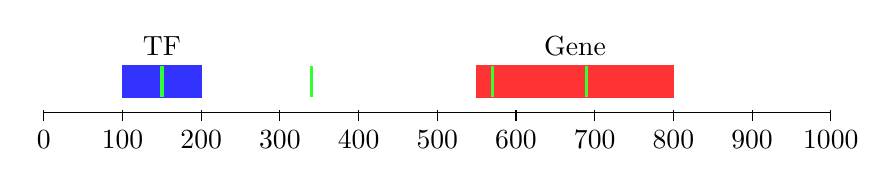
\begin{tikzpicture}[y=.2cm, x=.01cm]
  \draw (0, 0)  -- coordinate (x axis mid) (1000, 0);
  \foreach \x in {0,100,...,1000}
  \draw (\x,1pt) -- (\x,-3pt)
  node[anchor=north] {\x};

  \filldraw[draw=red!80, fill=red!80] (550, 1) rectangle ++(250,2) node[above=1, pos=0.5] {Gene};
  \filldraw[draw=blue!80, fill=blue!80] (100, 1) rectangle ++(100,2) node[above=1, pos=0.5] {TF};
  \foreach \x in {150, 340, 570, 690}
  \draw[color=green!80, very thick] (\x, 1) -- (\x, 3);
\end{tikzpicture}
\end{document}

%%% Local Variables:
%%% mode: latex
%%% TeX-master: t
%%% End:

%%% Local Variables:
%%% mode: latex
%%% TeX-master: t
%%% End:
